\documentclass[10pt,a4paper]{report}
\usepackage[utf8]{inputenc}
\usepackage[russian]{babel}
\usepackage{amsmath}
\usepackage{amsfonts}
\usepackage{amssymb}
\usepackage{graphicx}
\author{Кенть Никита}
\title{Лабораторная работа №4.\\
	Утилита Nmap}
\begin{document}
	\maketitle
	\tableofcontents
	\pagebreak
	
\section{Цель работы}
	Изучить возможности утилиты Nmap на различных примерах.
\section{Ход работы}
	Для выполненя данной лабораторной работы нам понадобятся две виртуальные машины: Metasplaitable2 и Kali Linux, имеющие адреса 192.168.32.128 и 192.168.32.129 соответственно. Конфигурации представлены на рис. \ref{pic:pic1} и рис. \ref{pic:pic2}
	
\begin{figure}[ht]	
	\center{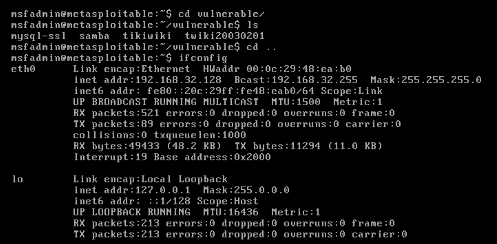
\includegraphics[width=0.8\linewidth]{pics/pic1}}
	\caption{Конфигурация Metasploitable2}
	\label{pic:pic1}
\end{figure} 


\begin{figure}[ht]	
	\center{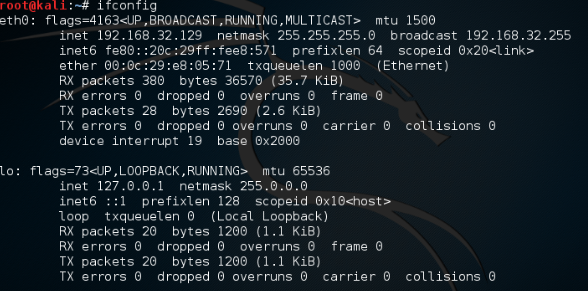
\includegraphics[width=0.8\linewidth]{pics/pic2}}
	\caption{Конфигурация Kali Linux}
	\label{pic:pic2}
\end{figure} 
\section{Поиск активных хостов}
Для поиска активных хостов запустим утилиту с флагом -sP и укажем адрeс подсети 192.168.32.*  Вывод утилиты приведет на рис.  \ref{pic:pic3}

\begin{figure}[ht]	
	\center{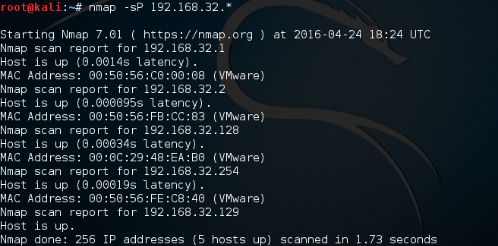
\includegraphics[width=0.8\linewidth]{pics/pic3}}
	\caption{Поиск активных хостов}
	\label{pic:pic3}
\end{figure} 
\section{Определение открытых портов}
Определим открытые порты, просто передав адрес хоста. (Рис. \ref{pic:pic4} )
\begin{figure}[ht]	
	\center{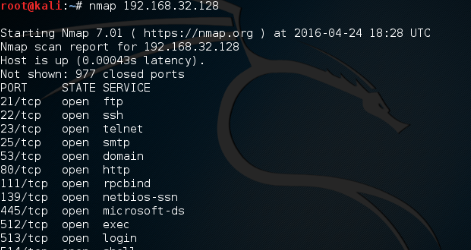
\includegraphics[width=0.8\linewidth]{pics/pic4}}
	\caption{Поиск открытых портов}
	\label{pic:pic4}
\end{figure} 
\section{Определение версии сервисов}
Определим версии сервисов, командой с ключем -sV (Рис. \ref{pic:pic5})
\begin{figure}[ht]	
	\center{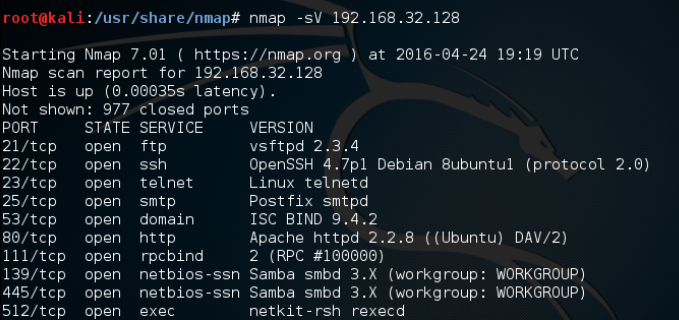
\includegraphics[width=0.8\linewidth]{pics/pic5}}
	\caption{Определение версии сервисов}
	\label{pic:pic5}
\end{figure} 


\section{Изучение nmap-services, nmap-os-db, nmap-service-probes}
\subsection{nmap-services}
Файл nmap-services содержит в себе описание назначения стандартных портов. Файл имеет структуру: имя\_сервиса, номер\_порта/название\_протокола, частота, комментарии. (Рис. \ref{pic:pic6})
			\begin{figure}[ht]	
	\center{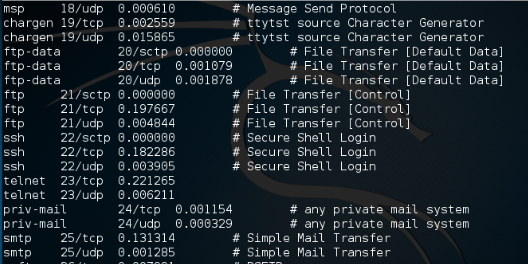
\includegraphics[width=0.8\linewidth]{pics/pic6}}
	\caption{nmap-services}
	\label{pic:pic6}
\end{figure} 

\subsection{nmap-os-db}
Файл содержит сигнатуры ответов различных операционных систем при сканировании. Это  Пример файла на рис. \ref{pic:pic7}

	\begin{figure}[ht]	
	\center{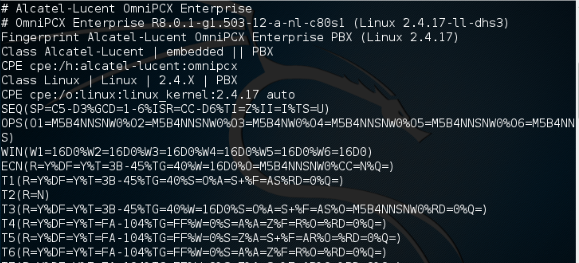
\includegraphics[width=0.8\linewidth]{pics/pic7}}
	\caption{nmap-os-db}
	\label{pic:pic7}
\end{figure} 		

\subsection{nmap-service-probes}
Файл содержит сигнатуры для определения сервисов, прослушивающих различные порты.Например, SMTP - почтовый сервер. Данные о сервисах задаются при помощи нескольких директив:
			\begin{itemize}
				\item Exclude <port specification>
				\item Probe <protocol> <probename> <probestring>
				\item match <service> <pattern> [<versioninfo>]
			\end{itemize}
			
\section{Добавление собственной сигнатуры в файл nmap-service-probes}
Для этого напишем небольшой сервер, который будем идентифицировать утилитой nmap
\begin{verbatim}
			#include <sys/types.h>
			#include <sys/socket.h>
			#include <netdb.h>
			#include <stdio.h>
			#include<string.h>
			
			int main()
			{
			
				char str[100];
				char *rec_srt="\x48\x65\x6c\x6c\x6f";
			
				int listen_fd, comm_fd;
			
				struct sockaddr_in servaddr;
			
				listen_fd = socket(AF_INET, SOCK_STREAM, 0);
			
				bzero( &servaddr, sizeof(servaddr));
			
				servaddr.sin_family = AF_INET;
				servaddr.sin_addr.s_addr = htons(INADDR_ANY);
				servaddr.sin_port = htons(22000);
			
				bind(listen_fd, (struct sockaddr *) &servaddr, sizeof(servaddr));
			
				listen(listen_fd, 10);
			
				comm_fd = accept(listen_fd, (struct sockaddr*) NULL, NULL);
			
				while(1)
				{
			
					bzero( str, 100);
			
					read(comm_fd,str,100);
			
					printf("echo back - %s",str);
			
					write(comm_fd, rec_srt, strlen(rec_srt)+1);
			
				}
			}
		\end{verbatim}		
Для определения данного сервера, в файл nmap-service-probes добавим:
\begin{verbatim}
			Probe TCP Server q|HelloServer|
			rarity 1
			ports 22000
			match testServer m|\x48\x65\x6c\x6c\x6f| v/1.0/
		\end{verbatim}	
Запустим сервис на машине Metasploitable2 и проверим с помощью nmap \begin{verbatim}
			root@kali:~/test# nmap 192.168.32.128 -p 22000 -sV
			
			Starting Nmap 7.01 ( https://nmap.org ) at 2016-03-20 19:33 EDT
			Nmap scan report for 192.168.202.2
			Host is up (0.00048s latency).
			PORT      STATE SERVICE    VERSION
			22000/tcp open  Server 1.0
		\end{verbatim}
	
\section{Сохранение вывода утилиты nmap в формате XML}
Для сохранения вывода утилиты nmap в формате  XML необходимо при запуске указать ключ "-oX". Часть содержания файла представлена на (Рис.\ref{pic:pic9})

			\begin{figure}[ht]	
	\center{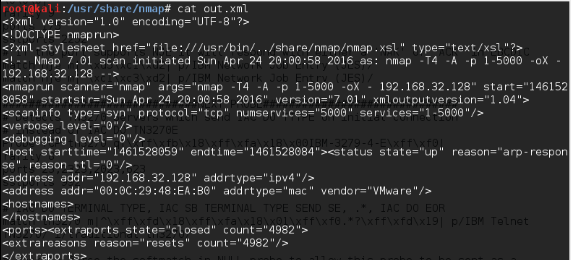
\includegraphics[width=0.8\linewidth]{pics/pic9}}
	\caption{Определение своего сервиса}
	\label{pic:pic9}
\end{figure} 	

\section{Исследование работы утилиты nmap при помощи wireshark}
Запустим WireShark и просканируем хост 192.168.32.128. Результаты на Рис. \ref{pic:pic10})

			\begin{figure}[ht]	
	\center{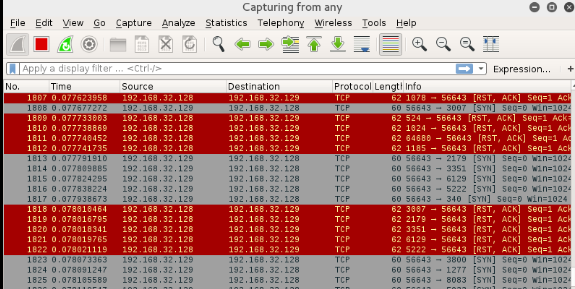
\includegraphics[width=0.8\linewidth]{pics/pic10}}
	\caption{WireShark}
	\label{pic:pic10}
\end{figure} 
\section{Использвоание db\_nmap из состава metasploit-framewor}
\begin{verbatim}
			root@kali:~# service postgresql start
			root@kali:~# msfdb init
			Creating database user 'msf'
			Enter password for new role: 
			Enter it again: 
			Creating databases 'msf' and 'msf_test'
			Creating configuration file in /usr/share/metasploit-framework/config/database.yml
			Creating initial database schema
		\end{verbatim}
		После чего необходимо запустить msfconsole и можно использовать любую из команд, описанных выше, но вместо nmap можно использовать db\_nmap. Результаты работы будут записаны в базу данных, тем самым обеспечивая экономию времени при сканировании портов.
\section{Анализ записей из файла nmap-service-probes}	
Рассмотрим строки, указанные на рис. \ref{pic:pic11})	

\begin{figure}[ht]	
	\center{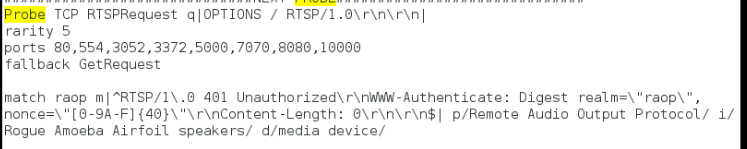
\includegraphics[width=0.8\linewidth]{pics/pic11}}
	\caption{Пример nmap-service-probes}
	\label{pic:pic11}
\end{figure} 
Директива Probe указывает, какое сообщение необходимо отправить для индентификации сервиса. В данном случае, сервис - RTSPRequest, протокол - TCP, отправляется следующая строка:
\begin{verbatim}
 OPTIONS / RTSP/1.0\r\n\r\n. 
\end{verbatim}
rarity указывает частоту, с которой от сервиса можно ожидать возвращения корректных результатов. В данном случае - 5. \\
Директивы ports и sslports указывают на порты, используемые данным сервисом. \\
fallback указывает на то, какие Probe необходимо использовать при отсутствии совпадений в текущей секции Probe. \\
Директива match необходима при распознавании сервиса на основе ответов на строку, отправленную предыдущей директивой Probe.
\section{Описание работы скрипта из Nmap}
Скриптовый движок Nmap (NSE) это одна из наиболее мощных и гибких возможностей Nmap. Он позволяет пользователям писать (и делиться ими) скрипты для автоматизации широкого круга сетевых задач. 
Рассмотрим скрипт  	dhcp-discover, который Обнаруживает сервера DHCP в сети. Запрос отправляется с UDP-порта 67, ответ принимается на порт 68.
\begin{verbatim}
 nmap -sU -p 67 --script=dhcp-discover <target>
 
 Возможный вывод скрипта:
 Interesting ports on 192.168.1.1:
PORT   STATE SERVICE
67/udp open  dhcps
| dhcp-discover:
|   DHCP Message Type: DHCPACK
|   Server Identifier: 192.168.1.1
|   IP Address Lease Time: 1 day, 0:00:00
|   Subnet Mask: 255.255.255.0
|   Router: 192.168.1.1
|_  Domain Name Server: 208.81.7.10, 208.81.7.14
\end{verbatim}
Приведем листинг скрипта:
\begin{verbatim}


author = "Ron Bowes"

license = "Same as Nmap--See https://nmap.org/book/man-legal.html"

categories = {"discovery", "safe"}


-- We want to run against a specific host if UDP/67 is open
function portrule(host, port)
  if nmap.address_family() ~= 'inet' then
    stdnse.debug1("is IPv4 compatible only.")
    return false
  end

  return shortport.portnumber(67, "udp")(host, port)
end

local function go(host, port)

  -- Build and send a DHCP request using the specified request type, or DHCPINFORM
  local requests = tonumber(nmap.registry.args.requests or 1)
  local results = {}
  for i = 1, requests, 1 do
    -- Decide which type of request to make
    local request_type = dhcp.request_types[nmap.registry.args.dhcptype or "DHCPINFORM"]
    if(request_type == nil) then
      return false, "Valid request types: " .. stdnse.strjoin(", ", dhcp.request_types_str)
    end

    -- Generate the MAC address, if it's random
    local mac_addr = host.mac_addr_src
    if(nmap.registry.args.randomize_mac == 'true' or nmap.registry.args.randomize_mac == '1') then
      stdnse.debug2("Generating a random MAC address")
      mac_addr = {}
      for j=1, 6, 1 do
        mac_addr[i] = string.char(math.random(1, 255))
      end
      mac_addr = table.concat(mac_addr)
    end

    local iface, err = nmap.get_interface_info(host.interface)
    if ( not(iface) or not(iface.address) ) then
      return false, "Couldn't determine local ip for interface: " .. host.interface
    end

    local status, result = dhcp.make_request(host.ip, request_type, iface.address, mac_addr)
    if( not(status) ) then
      stdnse.debug1("Couldn't send DHCP request: %s", result)
      return false, result
    end

    table.insert(results, result)
  end

  -- Done!
  return true, results
end

local commasep = {
  __tostring = function (t)
    return table.concat(t, ", ")
  end
}

action = function(host, port)
  local status, results = go(host, port)


  if(not(status)) then
    return stdnse.format_output(false, results)
  end

  if(not(results)) then
    return nil
  end

  -- Set the port state to open
  if(host) then
    nmap.set_port_state(host, port, "open")
  end

  local response = stdnse.output_table()

  -- Display the results
  for i, result in ipairs(results) do
    local result_table = stdnse.output_table()

    if ( nmap.registry.args.dhcptype and
      "DHCPINFORM" ~= nmap.registry.args.dhcptype ) then
      result_table["IP Offered"] = result.yiaddr_str
    end
    for _, v in ipairs(result.options) do
      if(type(v.value) == 'table') then
        setmetatable(v.value, commasep)
      end
      result_table[ v.name ] = v.value
    end

    if(#results == 1) then
      response = result_table
    else
      response[string.format("Response %d of %d", i, #results)] = result_table
    end
  end

  return response
end
\end{verbatim}
\section{Вывод}
В ходе лабораторной работы была изучена утилита Nmap. Попробовали некоторые её возможности, такие как: поиск активных хостов, открытых портов,версий сервисов и др. Изучены файлы nmap-services, nmap-os-db, nmap-service-probe. Идентифицировали собственный сервис.
\end{document}